\documentclass[aspectratio=169,11pt]{beamer}

\usepackage[T1]{fontenc}
\usepackage{lmodern}
\usepackage{amsmath,amssymb}
\usepackage{graphicx}

\definecolor{Ink}{HTML}{16283A}
\definecolor{Teal}{HTML}{087F8C}
\definecolor{Coral}{HTML}{D95D39}
\definecolor{Paper}{HTML}{F7F4EE}
\definecolor{Muted}{HTML}{526475}

\setbeamercolor{normal text}{fg=Ink,bg=Paper}
\setbeamercolor{frametitle}{fg=Ink,bg=Paper}
\setbeamercolor{structure}{fg=Teal}
\setbeamercolor{alerted text}{fg=Coral}
\setbeamercolor{title}{fg=Paper}
\setbeamercolor{subtitle}{fg=Paper}
\setbeamercolor{author}{fg=Paper}
\setbeamercolor{date}{fg=Paper}
\setbeamerfont{title}{series=\bfseries,size=\fontsize{27}{31}}
\setbeamerfont{subtitle}{size=\normalsize}
\setbeamerfont{frametitle}{series=\bfseries,size=\fontsize{21}{24}}
\setbeamerfont{normal text}{size=\normalsize}
\setbeamertemplate{navigation symbols}{}
\setbeamersize{text margin left=0.65cm,text margin right=0.65cm}

\setbeamertemplate{frametitle}{
  \vspace{0.30cm}
  \insertframetitle\par
  \vspace{0.08cm}
  {\color{Teal}\rule{\textwidth}{0.8pt}}
}

\setbeamertemplate{footline}{
  \leavevmode
  \hbox{%
    \begin{beamercolorbox}[wd=.88\paperwidth,ht=2.8ex,dp=1.2ex,leftskip=.65cm]{normal text}
      \scriptsize\color{Muted}\texttt{github.com/amchavezu/ai-04-acemoglu}
    \end{beamercolorbox}%
    \begin{beamercolorbox}[wd=.12\paperwidth,ht=2.8ex,dp=1.2ex,center]{normal text}
      \scriptsize\color{Muted}\insertframenumber/5
    \end{beamercolorbox}%
  }
}

\newcommand{\key}[1]{\textcolor{Teal}{\textbf{#1}}}
\newcommand{\caveat}[1]{\textcolor{Coral}{\textbf{#1}}}

\title{AI, Human Cognition and\\Knowledge Collapse}
\subtitle{Daron Acemoglu, Dingwen Kong, and Asuman Ozdaglar\\
NBER Working Paper 34910, primary version: May 5, 2026}
\author{Alvaro Marcelo Chávez Unyen}
\date{\texttt{github.com/amchavezu/ai-04-acemoglu}}

\begin{document}

{
\setbeamercolor{background canvas}{bg=Ink}
\begin{frame}[plain]
  \vspace{0.65cm}
  {\usebeamerfont{title}\color{Paper}\inserttitle\par}
  \vspace{0.45cm}
  {\usebeamerfont{subtitle}\color{Paper}\insertsubtitle\par}
  \vfill
  {\large\color{Paper}\insertauthor\par}
  \vspace{0.12cm}
  {\small\color{Paper}\insertdate\par}
  \vspace{0.45cm}
\end{frame}
}

\begin{frame}{The paper and the agent's problem}
\begin{columns}[T,totalwidth=\textwidth]
\begin{column}{0.40\textwidth}
  \key{Question}\\[0.10cm]
  Can better personalized AI decisions today weaken the human effort that
  maintains collective knowledge tomorrow?

  \vspace{0.15cm}
  \key{Two complementary inputs}
  \begin{itemize}\setlength\itemsep{0.05cm}
    \item General knowledge: \(X\) about the common state
    \item Context-specific knowledge: \(Y\) about the current case
  \end{itemize}
\end{column}
\begin{column}{0.57\textwidth}
  {\small
  \[
  \max_{e\geq0}
  \left\{
  \begin{aligned}
  &f(0,0)+G(X)\Delta_G+G(X)G(Y)\Delta_X\\
  &-\frac{\varepsilon}{\varepsilon+1}
    e^{(\varepsilon+1)/\varepsilon}
  \end{aligned}
  \right\}
  \]
  }
  \[
  Y=\sigma^{-2}+\lambda_Ie+\tau_A
  \]
  Effort and AI both raise private precision \(Y\).
\end{column}
\end{columns}

\vfill
{\color{Coral}\rule{\textwidth}{0.8pt}}\\[-0.04cm]
{\small\textbf{Externality.} The agent captures the private return to effort,
but not the general knowledge contributed to future cohorts.}
\end{frame}

\begin{frame}{Main result and conditions}
\begin{columns}[T,totalwidth=\textwidth]
\begin{column}{0.53\textwidth}
  \[
  U_{eX}
  =\lambda_I\Delta_Xg(X)g(Y)>0
  \]
  \[
  U_{e\tau_A}
  =\lambda_I\Delta_XG(X)g'(Y)<0
  \]

  \[
  \boxed{
  X>0,\;Y>0,\;\Delta_X>0,\;
  \lambda_I>0,\;\varepsilon>0
  }
  \]
\end{column}
\begin{column}{0.44\textwidth}
  \key{General knowledge complements effort}\\
  Better common-state knowledge raises the value of learning about the
  particular case.

  \vspace{0.25cm}
  \key{Agentic AI substitutes for effort}\\
  Both raise \(Y\). Since \(g'(Y)<0\), AI lowers the marginal return to human
  learning.
\end{column}
\end{columns}

\vfill
\caveat{Boundary note.} At \(X=0\), \(U_{e\tau_A}=0\) and \(g(0)\) is not
finite. The strict cross-partials are interior statements.
\end{frame}

\begin{frame}{What I did}
\begin{columns}[T,totalwidth=\textwidth]
\begin{column}{0.44\textwidth}
  \key{1. Audited Observation 1}\\[0.08cm]
  The economic mechanism is correct. Its strict derivative formulation
  requires \(X>0\). Discrete differences preserve the global interpretation
  weakly.

  \vspace{0.35cm}
  \key{2. Relaxed \(\Delta_I=0\)}\\[0.08cm]
  Context-specific correctness now has value even when general knowledge is
  absent.
\end{column}
\begin{column}{0.53\textwidth}
  \[
  \begin{aligned}
  U_e={}&\lambda_Ig(Y)
  [\Delta_I+G(X)\Delta_X]\\
  &-e^{1/\varepsilon}
  \end{aligned}
  \]

  \[
  \begin{gathered}
  \Delta_I>0
  \Rightarrow e_\Delta(0,\tau_A)>0\\
  \Rightarrow F_\Delta(0)>0
  \end{gathered}
  \]

  \vspace{0.18cm}
  \caveat{Implication}\\
  Complete zero-knowledge collapse disappears, but low-knowledge steady states
  remain an open question.
\end{column}
\end{columns}
\end{frame}

\begin{frame}{Where I did not believe the AI}
\begin{columns}[T,totalwidth=\textwidth]
\begin{column}{0.55\textwidth}
  \centering
  \IfFileExists{hand/observation1-boundary.jpg}{
    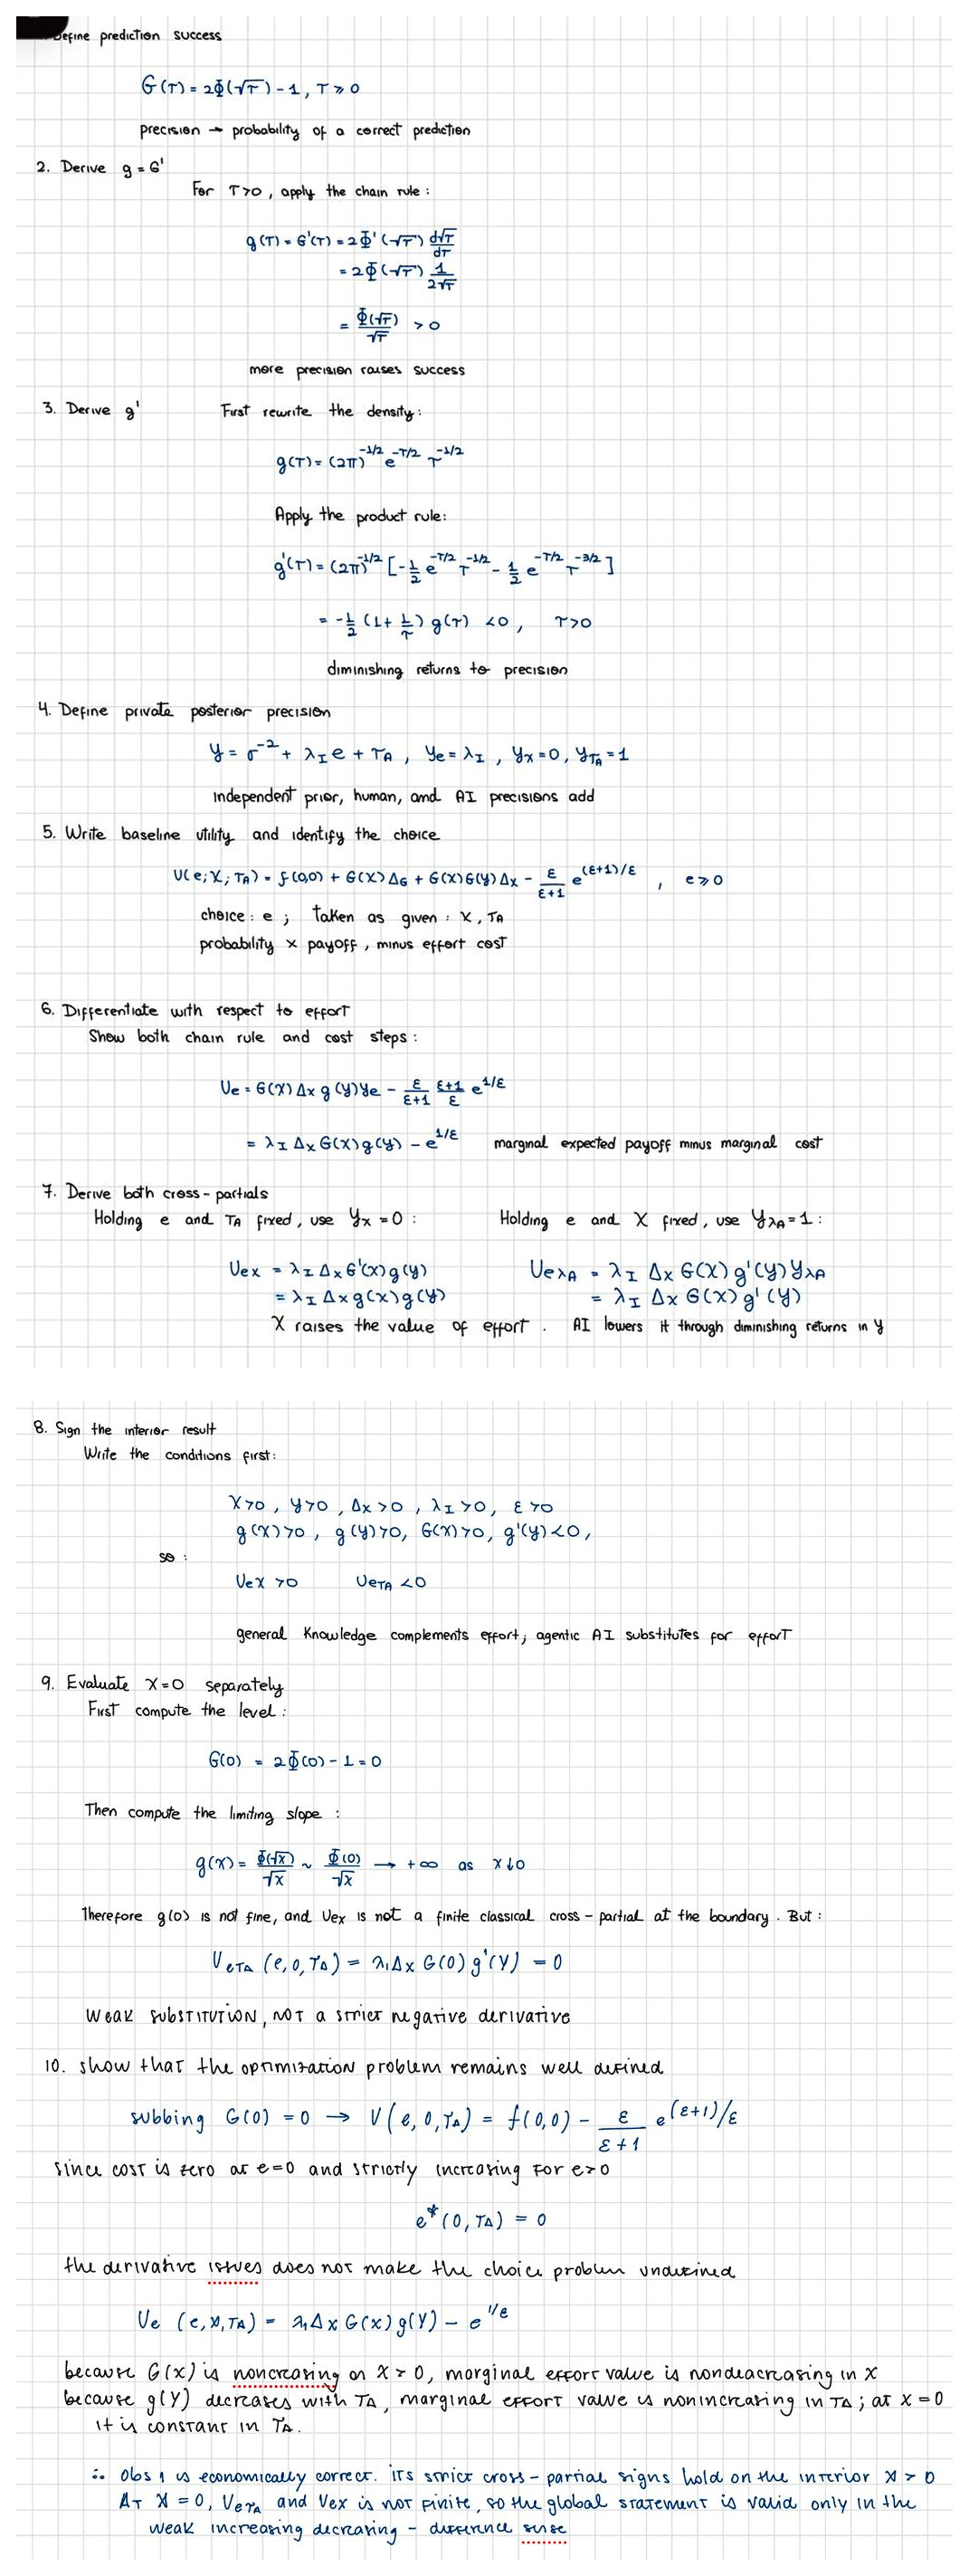
\includegraphics[width=\linewidth,height=0.70\textheight,keepaspectratio]
    {hand/observation1-boundary.jpg}
  }{
    \fbox{
      \parbox[c][0.58\textheight][c]{0.88\linewidth}{
        \centering
        {\Large\color{Coral}\textbf{PENDING STUDENT PHOTO}}\\[0.25cm]
        \normalsize
        \texttt{hand/observation1-boundary.jpg}\\[0.18cm]
        Cross-partials and the \(X=0\) boundary check
      }
    }
  }
\end{column}
\begin{column}{0.42\textwidth}
  \key{Initial claim}\\
  Both cross-partials are strictly signed globally.

  \vspace{0.30cm}
  \key{Hand check}\\
  At \(X=0\),
  \[
  U_{e\tau_A}=0,
  \qquad g(0)\notin\mathbb R.
  \]

  \vspace{0.16cm}
  \key{Verdict}\\
  Correct on the interior, incomplete at the boundary. The mechanism remains
  economically valid in a weak global sense.
\end{column}
\end{columns}
\end{frame}

\end{document}
